\documentclass[11pt,a4paper]{article}

\usepackage[T1]{fontenc}
\usepackage[utf8]{inputenc}
\usepackage{mathptmx}
\usepackage{courier}
\usepackage[margin=2.5cm]{geometry}
\usepackage{amsmath}
\usepackage{booktabs}
\usepackage{graphicx}
\usepackage{xcolor}
\usepackage[numbers,sort&compress]{natbib}
\usepackage{xurl}
\usepackage[hidelinks]{hyperref}
\hypersetup{pdftitle={Give the Model the Overlap, Not the Dates: Tool Evidence for Checking Time-Qualified Claims with Small Local Models},pdfauthor={Muzammal Hussain}}
\usepackage{caption}
\captionsetup{font=small,labelfont=bf}

\newcommand{\code}[1]{\texttt{#1}}
\setlength{\emergencystretch}{3em}

\title{\textbf{Give the Model the Overlap, Not the Dates:\\Tool Evidence for Checking Time-Qualified Claims\\with Small Local Models}}
\author{Muzammal Hussain\\
\small Independent researcher, Glasgow, United Kingdom\\
\small \href{mailto:muzammal@masmatixinnovations.co.uk}{muzammal@masmatixinnovations.co.uk}\\
\small ORCID: \href{https://orcid.org/0009-0001-2570-5686}{0009-0001-2570-5686}}
\date{\small November 2026}

\begin{document}
\maketitle

\begin{abstract}
\noindent
A claim such as ``X was president of Y in 1865'' is right, wrong or partly right depending on whether the stated time
lies inside, outside or across the period in which the fact held. We ask what a small local model needs from its
tools to make this call. On 150 claims from TimeStress, balanced over the three labels, two models run with Ollama
(\code{qwen2.5:3b} and \code{llama3.1:8b}) answered under three conditions on the same rows: from memory, with a tool
that returns the claim's time span and the fact's validity period, and with a tool that also returns overlap flags.
From memory the models reached 35.3\% and 46.0\% accuracy, close to the 33.3\% of guessing. Given the two date spans,
\code{qwen2.5:3b} still labelled almost every claim as wrong (41.3\%). \code{llama3.1:8b} scored 30.0\% under strict
scoring because it ended 79 of 150 episodes with a malformed final action; scoring those answers anyway gives 72.0\%,
with every claim inside the period right but only 36\% of the partly overlapping claims. With the overlap flags both
models reached 98.7--100\%. Asked instead to write the comparison as a Python expression over the dates, they almost
never produced code that ran (0 and 6 of 150 claims); with a syntax example and one chance to repair, \code{llama3.1:8b}
ran code on 110 claims but its logic was right on only 47 (31.3\%); \code{qwen2.5:3b} ran code on 6 claims and was right on 2. The hard step is comparing intervals, above all at the boundary, and code does it
exactly. Tool-using agents for temporal checks should compute the comparison in code and leave the model to read and
report it, and evaluations should report protocol errors separately from wrong answers.
\end{abstract}

\section{Introduction}

Many facts hold only for a period: an office, a marriage, a club membership. A statement that places such a fact at
a time is right when that time lies inside the period, wrong when it lies outside, and partly right when it crosses a
boundary. TimeStress~\cite{khodja2025timestress} turns Wikidata facts into such statements at year, month and day
precision and shows that language models often fail to tell right contexts from wrong ones when they answer from
memory.

An agent does not have to answer from memory. It can look up the fact's validity period and compare it with the time
in the claim. This splits the task into two parts: \emph{retrieving} the period, which a tool can do exactly, and
\emph{comparing} two intervals, which a model or code can do. Work on tool use and program-aided reasoning suggests
that models are weak at exactly this kind of comparison and arithmetic and that offloading it helps
\cite{schick2023toolformer,gao2023pal}. We measure how much it matters for small models that a clinic, a newsroom
or a records office could run locally.

We hold the claims, labels and prompts fixed and change only what the tool returns: nothing (memory only), the two
date spans, or the spans plus overlap flags, and in two further conditions ask the model to write the comparison
itself as code. Our contributions:
\begin{itemize}
  \item A paired comparison of the three evidence levels for two small local models on 150 TimeStress claims balanced
  over labels, with fact-level bootstrap intervals and exact McNemar tests.
  \item Evidence that the bottleneck is the interval comparison, not the lookup: given the dates, one model still
  answered ``incorrect'' for 37 of 50 right claims, and the other recognised only 36\% of the partly overlapping claims.
  \item Evidence that model-written code is not a substitute: asked to compute the comparison in a Python expression,
  the models rarely produced code that ran, and after one repair \code{llama3.1:8b}'s code ran on 110 claims but
  encoded the wrong interval logic, right on only 31.3\% of all claims.
  \item A strict and a lenient score for each condition, showing that a protocol error (a misnamed final action) can
  hide most of a model's correct judgements.
\end{itemize}

\section{Related work}

\paragraph{Temporal knowledge and reasoning.} TimeQA~\cite{chen2021timeqa} built time-sensitive questions from
Wikidata facts aligned with Wikipedia. TempReason~\cite{tan2023tempreason} probes time--time, time--event and
event--event reasoning and finds a large gap to human performance. Test of Time~\cite{fatemi2025testoftime} uses
synthetic data to separate the semantics of time from time arithmetic, so that results do not depend on facts seen
in pre-training. TimeStress~\cite{khodja2025timestress}, which we use, asks whether models recall the same fact
across many temporal contexts and reports low robustness. These works evaluate models answering from memory or from
text; we keep TimeStress's labels and give the model tools.

\paragraph{Tools and code for reasoning.} Toolformer~\cite{schick2023toolformer} trains a model to call APIs, among
them a calculator, for the basic operations where language models are weak. PAL~\cite{gao2023pal} lets the model write
a program and leaves the solution step to an interpreter. ReAct~\cite{yao2023react} interleaves reasoning with tool
actions. Our tool conditions follow the same idea in its simplest form: the comparison is done either by the model or
by code, and we measure the difference.

Artefacts in LLM-optimised evidence for multilingual fact-checking are analysed in \cite{hussain2026civintel}, and the verification of treaty-status claims against official records in \cite{hussain2026treaty}.

\section{Method}

\paragraph{Data.} TimeStress~\cite{khodja2025timestress} (file \code{train.parquet}, revision \code{f90d17c},
CC BY-SA 4.0) pairs each fact with time contexts and a label: \emph{correct} if the context lies inside the fact's
validity period, \emph{incorrect} if it does not overlap it, and \emph{transitional} if it partly overlaps it. Rows
without a usable context, and rows whose dates fall before year 1 and cannot be represented, were excluded, leaving
500,108 rows from 1,982 facts (431,943 incorrect, 66,651 correct, 1,514 transitional). In TimeStress every
transitional row has year precision.

\paragraph{Reference policies.} Predicting the majority label (\emph{incorrect}) gives 86.4\% accuracy on all rows.
An interval rule that compares the context with the validity period gives 100\%, because it applies the definition
that produced the labels; it is a ceiling, not a competitor.

\paragraph{Agent sample.} Because the data are dominated by \emph{incorrect}, the agents were run on a balanced sample
of 150 rows, 50 per label, drawn with a fixed seed and spread over precisions within each label (82 year, 34 month and
34 day rows; all 50 transitional rows are years). The 150 rows come from 82 facts. Both models saw the same rows.

\paragraph{Conditions.} All three conditions use the same label definitions in the system prompt. \emph{Text only}:
the model sees the statement and answers from memory. \emph{Tool: dates}: the agent must call
\code{get\_fact\_interval}, then \code{compare\_context}, which returns the context span and the validity period, and
then give a final answer; the agent has to compare the two spans itself. \emph{Tool: dates, write code}: after the
same two calls the agent must return a one-line Python expression over the six dates that evaluates to the label; a
restricted evaluator (comparisons, \code{and}/\code{or}, conditional expressions and string constants only) runs it.
\emph{With one repair}: the prompt adds one worked syntax example, and an expression that fails to parse or evaluate
is returned with the error for one corrected attempt. The code conditions were run in a second session with
replies constrained by a JSON schema that allows only the action expected at each step (Ollama structured output);
in that session we also re-ran the other three conditions. \emph{Tool: dates + overlap flags}: the same
loop, but \code{compare\_context} also returns the overlap in days and three flags (fully contained, no overlap,
partial overlap), from which the label follows directly. The agent loop allows three steps; a response that is not
the expected action ends the episode as an abstention.

\paragraph{Models and scoring.} \code{qwen2.5:3b}~\cite{qwen2025qwen25} and \code{llama3.1:8b}~\cite{grattafiori2024llama3}
ran through Ollama with temperature 0 and JSON output on a MacBook (Apple M4, 16 GB). Accuracy counts abstentions as
wrong. Because some abstentions were protocol errors after both tools had been called, we also report a
\emph{lenient} score that accepts a valid label given with a misnamed final action. Intervals are 95\% percentile
intervals from 10,000 bootstrap resamples of whole facts~\cite{efron1993bootstrap}; conditions are compared on the same
rows with exact McNemar tests.

\section{Results}

\begin{table}[t]
\centering
\small
\caption{Accuracy on the 150 balanced claims (50 per label). Abstentions count as wrong. 95\% fact-level bootstrap
intervals in brackets. ``Lenient'' accepts a valid label given with a misnamed final action. ``Transitional recall'': share of the 50 partly overlapping claims labelled transitional (lenient). Guessing gives 33.3\%.}
\label{tab:main}
\setlength{\tabcolsep}{3pt}
\begin{tabular}{llrrrr}
\toprule
Model & Condition & Accuracy (\%) & Abstained & Lenient (\%) & Transitional recall \\
\midrule
\code{qwen2.5:3b} & Text only & 35.3 [22.8, 47.2] & 0 & 35.3 & 0\% \\
 & Tool: dates & 41.3 [29.2, 52.7] & 1 & 41.3 & 4\% \\
 & Tool: dates + overlap flags & 98.7 [96.6, 100.0] & 1 & 98.7 & 98\% \\
 & Tool: dates, write code & 0.0 & 150 & 0.0 & 0\% \\
 & \quad with one repair & 1.3 [0.0, 3.4] & 144 & 1.3 & 2\% \\
\midrule
\code{llama3.1:8b} & Text only & 46.0 [33.8, 57.7] & 0 & 46.0 & 10\% \\
 & Tool: dates & 30.0 [21.0, 39.7] & 79 & 72.0 & 36\% \\
 & Tool: dates + overlap flags & 88.7 [80.9, 95.6] & 17 & 100.0 & 100\% \\
 & Tool: dates, write code & 2.7 & 144 & 2.7 & 8\% \\
 & \quad with one repair & 31.3 [23.3, 39.5] & 40 & 31.3 & 26\% \\
\bottomrule
\end{tabular}
\end{table}

\begin{figure}[t]
  \centering
  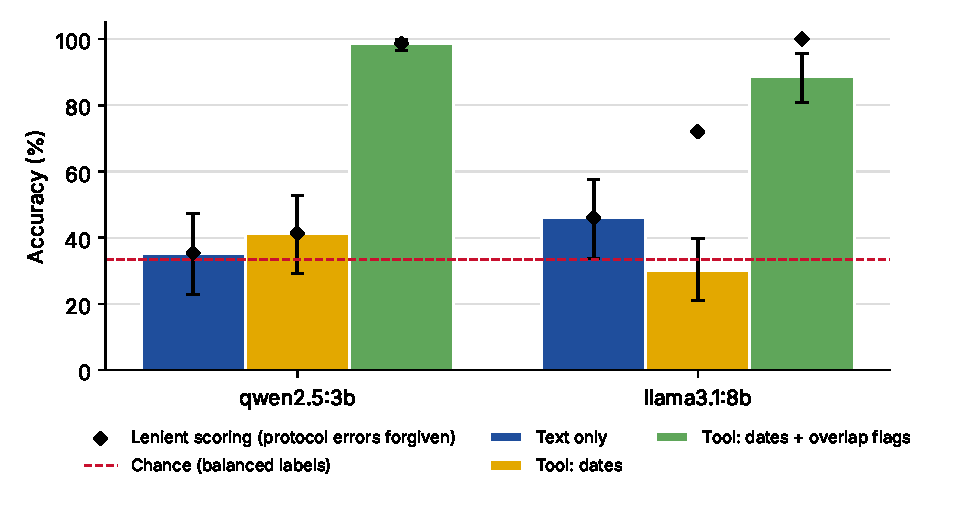
\includegraphics[width=0.82\linewidth]{figures/fig_agent_accuracy.pdf}
  \caption{Accuracy by model and condition with 95\% fact-level bootstrap intervals. Diamonds: lenient score.
  Dashed line: guessing among three balanced labels.}
  \label{fig:accuracy}
\end{figure}

\paragraph{From memory, both models are close to guessing.} \code{qwen2.5:3b} answered \emph{incorrect} for 138 of
150 claims, including 45 of the 50 correct ones (35.3\%). \code{llama3.1:8b} spread its answers but called 39 of the
50 transitional claims correct (46.0\%). Neither model recognised partial overlap from memory (0\% and 10\%).

\paragraph{Given the dates, the comparison fails.} With both spans in hand, \code{qwen2.5:3b} improved only from
35.3\% to 41.3\% (11 rows gained, 2 lost; McNemar $p=0.022$). It still labelled 37 of 50 correct claims and 47 of 50
transitional claims as incorrect: it read the dates but did not compare them. \code{llama3.1:8b} scored 30.0\% under
strict scoring, below its memory-only score ($p=0.005$), because 79 episodes ended with the action
\code{classify} instead of \code{final}. In every one of these episodes both tools had already been called, and 63 of
the 79 labels were right. Scored leniently, \code{llama3.1:8b} reached 72.0\% [62.3, 80.4], well above memory alone
(47 rows gained, 8 lost; $p<10^{-7}$). It was right on all 50 claims inside the period and on 80\% of those outside it,
but on only 18 of the 50 partly overlapping claims; it called 28 of them correct.

\paragraph{With overlap flags, both models are near the ceiling.} \code{qwen2.5:3b} reached 98.7\% and
\code{llama3.1:8b} 88.7\% under strict scoring and 100\% leniently; its 17 strict errors were again misnamed final
actions with the right label. Against the dates-only condition the flags gained 86 rows and lost none for
\code{qwen2.5:3b}, and 88 rows and lost none for \code{llama3.1:8b} ($p<10^{-25}$ for both). Per-precision accuracy is not reported as a separate finding, because in TimeStress all partly overlapping claims have year precision, so
precision and label cannot be separated.

\paragraph{Writing the comparison in code does not help.} When the agents had to express the comparison as a Python
expression, \code{qwen2.5:3b} produced no expression that ran and \code{llama3.1:8b} only 6 (Table~\ref{tab:main}).
The failures were syntax, not the evaluator: statements such as \code{if \ldots: \ldots} instead of an expression, date
literals with leading zeros, undefined names and expressions that returned no label. With a worked example and one repair,
\code{llama3.1:8b} produced running code on 110 claims (105 of them after the repair), but the label was right on only
47; it called 48 claims correct, including 18 of the 50 partly overlapping and 9 of the 50 outside the period. Its
expressions ran but encoded the wrong interval logic, for example treating any overlap as \emph{correct} or labelling
containment as \emph{transitional}. \code{qwen2.5:3b} still failed on 144 claims.
Delegating the comparison to model-written code therefore moves the error from arithmetic to logic; the code has to be
written by the tool's author, not by the model.

\section{Discussion}

\paragraph{Where the error lies.} The three conditions separate three abilities. Memory alone was not enough, which
agrees with the low robustness reported for TimeStress~\cite{khodja2025timestress}. Looking up the period did not fix
this either, because the small models could not reliably decide how two date spans relate, and failed most on the
partial overlap that defines a transitional claim. Once code had computed the overlap, the models only had to read a
flag, and both did so almost perfectly; when the models had to write that code themselves, they failed at syntax and,
after a repair, at the logic of interval overlap. The practical rule is the one behind program-aided
reasoning~\cite{gao2023pal}: a tool for temporal checks should return the comparison, not only the inputs to it.

\paragraph{The flags condition is not a reasoning test.} With overlap flags the label follows by rule, so 98.7--100\%
shows that the models copy a well-defined signal, not that they reason about time. Its value is as the operating
point of a well-designed tool: it tells a builder what accuracy to expect when the comparison is done in code.

\paragraph{Strict and lenient scores answer different questions.} Strict scoring measures whether an agent follows
the tool protocol; lenient scoring measures whether its judgement is right. For \code{llama3.1:8b} the two differ by
42 points in the dates condition, and the strict score alone would have suggested that dates make the model worse.
Agent evaluations should report both, or constrain the output format so that the distinction cannot arise. We
checked the second option: with schema-constrained replies \code{llama3.1:8b} made no protocol errors and scored
72.7\% with dates and 100\% with overlap flags, matching its lenient scores (72.0\% and 100\%); \code{qwen2.5:3b}
scored exactly as before (35.3\%, 41.3\%, 98.7\%).

\section{Limitations}

The agent sample has 150 claims from 82 facts, so intervals are wide (about $\pm$12 points for the memory and dates
conditions). Two small models were tested, once each, at temperature 0, with one prompt per condition (the code conditions were
run in a later session on the same rows); larger models,
other prompts or a chain-of-thought step may compare dates better. All transitional claims have year precision, so
partial overlap was only tested at that precision. The labels are TimeStress's interval labels, which follow from
Wikidata validity periods; they do not check whether the underlying historical fact is true. The lenient score
accepts a label only when it was given after both tool calls; a different parser could recover more or fewer answers.

\section{Conclusion}

Small local models asked whether a time-qualified claim holds were close to guessing from memory and barely better
when given the dates, because they could not reliably compare two date spans, above all at a boundary. When a tool
returned the overlap, both models reached 98.7--100\%; when they had to write the comparison in code, even with a
repair step, they reached at most 31.3\%. Temporal agents should do interval arithmetic in code, and
their evaluations should keep protocol errors apart from wrong answers.

\section*{Code and data availability}

Code, tests, the per-row agent predictions and tool traces for both models and all five conditions, the analysis script and the figure are
at \url{https://github.com/MHKhan50/ChronoFact-AgentBench} and archived on Zenodo
(\href{https://doi.org/10.5281/zenodo.24356041}{doi:10.5281/zenodo.24356041}, all versions). TimeStress is not redistributed; the pipeline downloads
the pinned file from Hugging Face and checks its SHA-256. Code is released under the MIT licence; TimeStress is
CC BY-SA 4.0.

\bibliographystyle{unsrtnat}
\bibliography{references}

\end{document}
